\newpage
\section{Eksamensopgave 8 - Vekselsstrøm}
\subsection{Kurven viser spændingsvariationer på en strømforsyning. Bestem maksimalspænidng, effektivspænding og frekvens.}
\begin{figure}[h!]
    \centering
    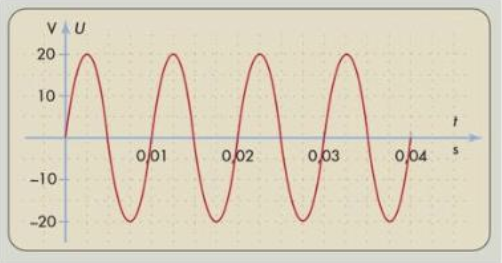
\includegraphics[width=0.5\textwidth]{figures/vekselsstrom.png}
    \caption{Kurve over vekselsstrøm}
\end{figure}
For at finde maks spænding \begin{math}U_{max}\end{math} kan vi kigge på den graf som vi har fået. På grafen kan vi se at den ikke går over 20V eller under 20V som betyder at maksimalspændingen er 20V\newline
For at finde effektivspænding kan vi bruge denne formel:
\begin{equation*}
    maximalspænding = \sqrt{2}\cdot effektivspænding
\end{equation*}
\begin{equation*}
    U_{max} = \sqrt{2}\cdot U_{eff}
\end{equation*}
Denne formel bruges til at finde maksimalspændingen med effektivspænding, men da vi allerede kender maksimalspændingen kan vi isolere effektivspænding ved at dividere med \begin{math}\sqrt{2}\end{math} på begge sider og beregne den ud fra den nye formel.
\begin{equation*}
    \frac{U_{maks}}{\sqrt{2}}=U_{eff}
\end{equation*}
\begin{equation*}
    U_{eff}=\frac{U_{maks}}{\sqrt{2}}
\end{equation*}
\begin{equation*}
    U_{eff}=\frac{20V}{\sqrt{2}}=14,14V
\end{equation*}
For at beregne frekvensen kan vi bruge denne formel
\begin{equation*}
    f=\frac{Antal Svingninger}{Tid}
\end{equation*}
På grafen kan vi se at den tager 1 svingning på 0,01 sekundt, derfor bliver formlen.
\begin{equation*}
    f=\frac{1}{0,01}=100Hz
\end{equation*}

\subsection{Spændingen tilkobles primærsiden på en transformer, der har 100 vindinger i primærspolen og 200 vindinger i sekundærspolen. Beregn spændingen på sekundærsiden.}
Til at beregne spændingen på sekundærsiden kan vi bruge denne formel
\begin{equation*}
    \frac{U_{s}}{U_{p}}=\frac{N_{s}}{N_{p}}
\end{equation*}
U står for spændingen\newline
N står for antal spoler\newline
S Står for sekundær\newline
P står for primær\newline
Med denne formel kan vi nu isolere \begin{math}U_{s}\end{math} ved at gange med \begin{math}U_{p}\end{math} på begge sider og indtaste værdierne.
\begin{equation*}
    U_{s}=U_{p}*\frac{N_{s}}{N_{p}}
\end{equation*}
\begin{equation*}
    U_{s}=20V*\frac{200}{100}=20V*2=40V
\end{equation*}

\subsection{Spændingen fra opgave a tilkobles en transmissionsledning på 100m med en modstand på 2,82 ohm. Der sendes 5 A gennem ledningen. Hvad bliver effekttabet i ledningen?}
\begin{equation*}
    P_{tab}=R\cdot I^{2}
\end{equation*}
\begin{equation*}
    P_{tab}=2,82\Omega\cdot 5^{2} A=2,82\Omega\cdot 25=70,5W
\end{equation*}

\newpage